\chapter{\IfLanguageName{dutch}{proof-of-concept}{proof-of-concept}}%
\label{ch:proof-of-concept}
\section{Inleiding}
In dit hoofdstuk bespreken we de implementatie van het proof-of-concept. We zullen elke fase van het proces in detail bespreken en de implementatie van de bijbehorende componenten toelichten. Hierbij zullen we ook de uitkomsten van elke fase beschrijven en hoe deze kunnen gebruikt worden in de volgende fase. \\

\section{Webscraper}
\subsection{Algemene Eisen}
Binnen de algemene eisen zal de webscraper voldoen aan de ethische aspecten \ref{subsection:scraper-ethische-aspecten} die zijn beschreven in de state of the art van dit onderzoek. Dit betekent dat de scraper de regels en richtlijnen van de gescrapte websites zal respecteren en zich zal houden aan eventuele beperkingen zoals vermeld in het robots.txt-bestand. Hierdoor wordt ervoor gezorgd dat de scrapingactiviteiten op een ethisch verantwoorde manier worden uitgevoerd. \\

Daarnaast zal de webscraper in staat zijn om verschillende websites te scrapen, met de focus op het verzamelen van de frontpage-inhoud. Specifiek zal de scraper de eerste 20 items van de frontpage van elke website verzamelen. \\

De webscraper zal twee bekende nieuwsbronnen scrapen, namelijk HLN en DeMorgen.

\subsection{Verkenning}
Alvorens we de webscraper kunnen implementeren, is het nodig om de DOM van beide websites te bekijken en een patroon hierin te herkennen. \\
\subsubsection{HLN}
Op de startpagina van HLN kunnen we zien (figuur \ref{fig:hln_frontpage}) dat elk nieuwsartikel zich bevindt binnen een article-tag bevindt. De eerste subtag is een a-tag met hierin de href naar het artikel. \\ Deze href zal belangrijk zijn om de datum te valideren en de titel te extraheren. We moeten deze dus opslaan. 

\begin{center}
    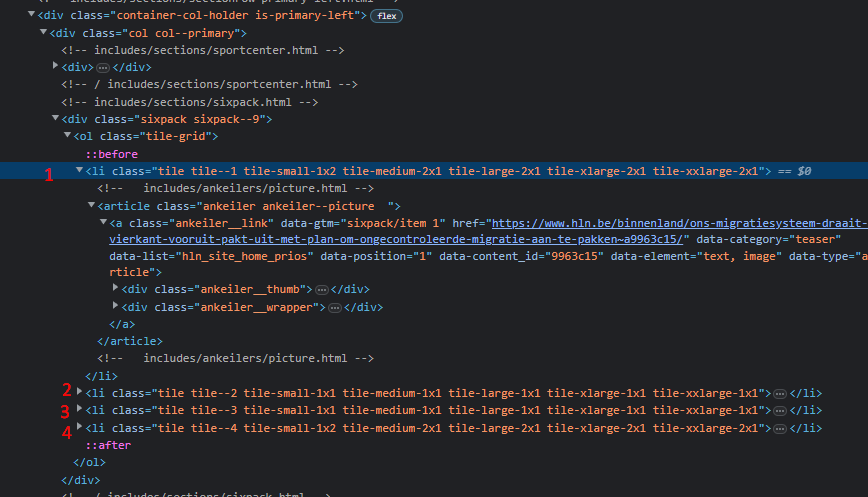
\includegraphics[width = 6in]{hln_frontpage2.png}
    \captionof{figure}{DOM van de startpagina van HLN met aangeduide nieuwsartikels.}
    \label{fig:hln_frontpage}
\end{center}

Als we vervolgens gaan kijken naar de DOM van een artikel, zien we dat de titel weergegeven wordt binnen een header-tag met als class 'article\_\_header' deze titel heeft als class 'article\_\_title'. De datum wordt weergegeven binnen een time-tag met datetime als value en class 'article\_\_time'. De datum is ook opgemaakt in een bepaald formaat, dd-mm-yy, hh:mm. Deze gegevens zijn essentieel voor de scraper. In figuur \ref{fig:hln_article} vind je dit terug. \\

\begin{center}
    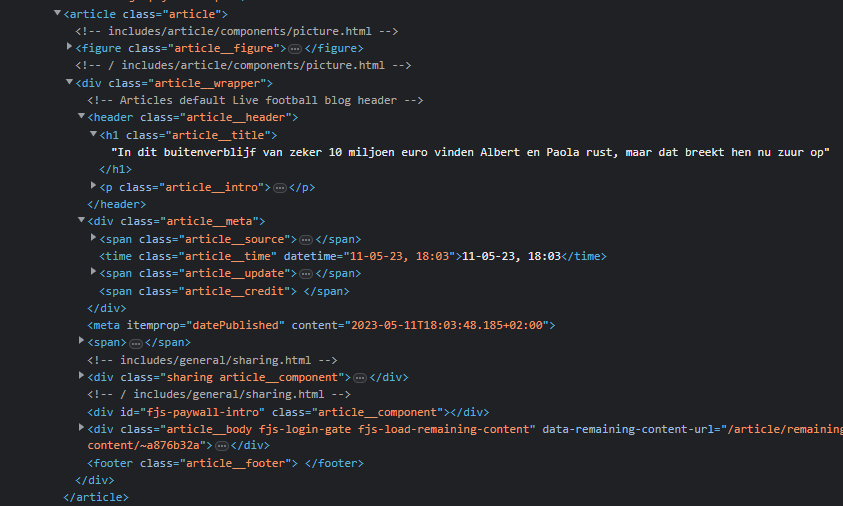
\includegraphics[width = 6in]{hln_article1.png}
    \captionof{figure}{DOM van een artikel op HLN met de essentiële elementen gemarkeerd.}
    \label{fig:hln_article}
\end{center}

\subsubsection{De Morgen}
De structuur van de artikels op de startpagina van De Morgen is vergelijkbaar met die van HLN. Zoals te zien is in figuur \ref{fig:demorgen_frontpage}, worden de artikels ook weergegeven binnen een article-tag, alleen is bij de morgen de tweede child de a-tag ten opzichte van HLN.

\begin{center}
    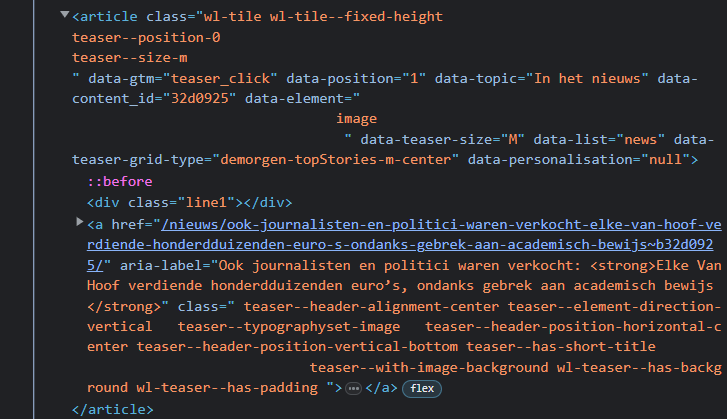
\includegraphics[width = 6in]{demorgen_frontpage2.png}
    \captionof{figure}{DOM van een artikel op De Morgen.}
    \label{fig:demorgen_frontpage}
\end{center}

Bij het doorklikken op een willekeurig artikel zien we dat de DOM vergelijkbaar is, maar niet exact hetzelfde qua structuur. In figuur \ref{fig:demorgen_article} zie je de DOM.

\begin{center}
    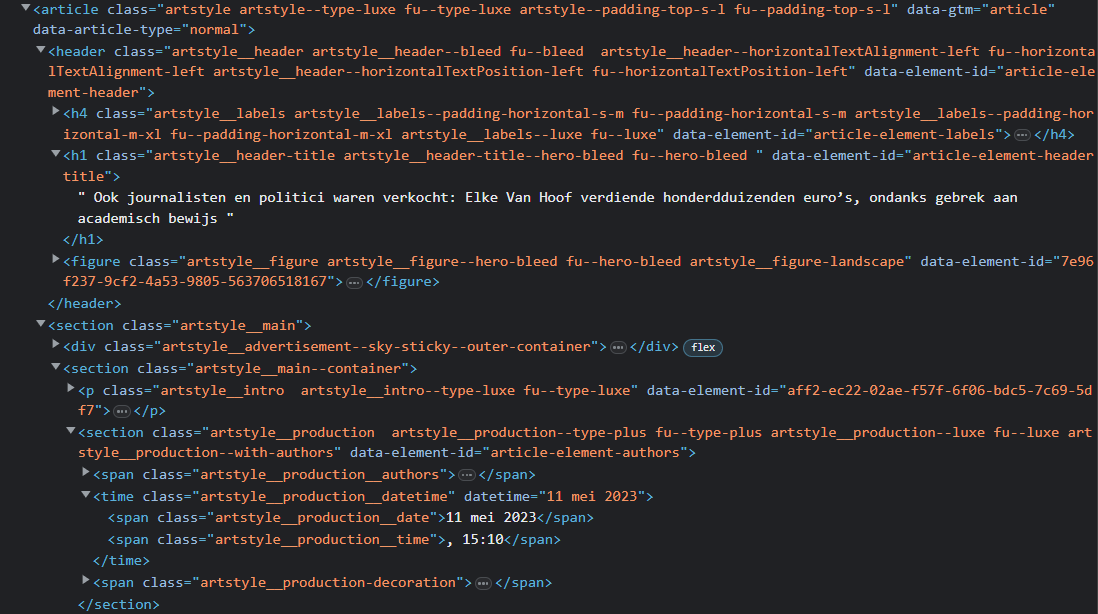
\includegraphics[width = 6in]{demorgen_article.png}
    \captionof{figure}{DOM van een artikel op De Morgen.}
    \label{fig:demorgen_article} 
\end{center}

Nu dat we deze informatie hebben. Kunnen we beginnen aan de implementatie van de scraper. 

\subsection{Implementatie}
\subsubsection{Thread-safe Dictionary}
Om ervoor te zorgen dat de gescrapete data veilig wordt opgeslagen, beginnen we de implementatie met het maken van een thread-safe dictionary.
\begin{pythoncode}{../../../workspace/src/scraper/util/volatileDictionary.py}
Deze thread-safe dictionary zal de opslag van de gescrapete data beheren en ervoor zorgen dat er geen problemen ontstaan tijdens het wegschrijven van de gescrapete data.
\end{pythoncode}

\subsubsection{Abstracte Thread}
Voordat we de specifieke threads implementeren, maken we eerst een AbstractThread-klasse die de methoden definieert die door de specifieke threads zullen worden gebruikt.

De AbstractThread-klasse bevat het volgende:

\begin{itemize}
    \item \textbf{Constructor}: Initialiseert de gemeenschappelijke eigenschappen die vereist zijn door de specifieke threads.
    \item \textbf{Methoden}: Definieert de gemeenschappelijke methoden die door de specifieke threads zullen worden gebruikt.
\end{itemize}

Laten we de \textbf{constructor} van de AbstractThread-klasse bespreken:

\begin{pythoncode}{../../../workspace/src/paper/abstractThreadCTR.py}
    In de constructor initialiseren we de gemeenschappelijke eigenschappen die vereist zijn door de specifieke threads. Deze eigenschappen omvatten:
\end{pythoncode}

    \begin{itemize}
        \item \textbf{dict}: De thread-safe dictionary die gebruikmaakt van dependency injection en geïnitialiseerd wordt.
        \item \textbf{limit}: De maximum waarde waarvan de artikels ouder moeten zijn.
        \item \textbf{articles}: De artikels die moeten worden verwerkt.
        \item \textbf{dateformat}: Het formaat van de datum dat wordt weergegeven in de artikelen.
        \item \textbf{title\_tag, title\_class, time\_tag, time\_class}: De HTML klassen waar de relevante gegevens in voorkomt.
        \item \textbf{base\_url}: De URL waarop de scraper moet starten.
        \item \textbf{routes}: De routes waarop de scraper toegestaan is te scrapen, rekening houdend met robots.txt terug te vinden op punt \ref{ch:liter_webscraping}.
        \item \textbf{headers}: De headers die aan de verzoeken worden toegevoegd om toegang te krijgen tot de website.
        \item \textbf{current}: Het momenteel verwerkte artikel.
        \item \textbf{article\_link}: De link van het huidige artikel dat overeenkomt met de opgegeven routes en momenteel wordt gescraped. \\
    \end{itemize}

Daarnaast bevat de AbstractThread-klasse ook verschillende methoden die het scrapen mogelijk maken. Laten we deze methoden bespreken:

\begin{pythoncode}{../../../workspace/src/paper/abstractThreadONSTART.py}
 Deze methode stuurt een initiële aanvraag naar de base\_url om de eerste 20 artikelen op te halen.
\end{pythoncode}

\begin{pythoncode}{../../../workspace/src/paper/abstractThreadSTARTSCRAPING.py}
Deze methode voert de on\_start()-methode uit, die de initiële artikelen ophaalt. Vervolgens gaat het door met het scrapen van artikelen zolang er artikelen in de lijst zijn. Elk artikel wordt gecontroleerd met behulp van de should\_scrape\_article()-methode en als het aan de voorwaarden voldoet, wordt het gescraped met behulp van de scrape\_article()-methode.
\end{pythoncode}

\begin{pythoncode}{../../../workspace/src/paper/abstractThreadSHOULDSCRAPE.py}
Deze methode controleert of de URL van een artikel overeenkomt met een van de opgegeven base\_urls. Als dit het geval is, wordt de article\_link ingesteld en wordt True geretourneerd om aan te geven dat het artikel moet worden gescraped.
\end{pythoncode}

\begin{pythoncode}{../../../workspace/src/paper/abstractThreadSCRAPE.py}
    Deze methode haalt de inhoud van de article\_link op met behulp van een GET-verzoek en de opgegeven headers. Vervolgens worden de datum en titel geëxtraheerd op basis van de opgegeven HTML-klassen. Als de geëxtraheerde datum vandaag is, wordt de append\_to\_dict()-methode aangeroepen om het artikel op te slaan in de thread-safe dictionary. \\
    
    Na elke request naar een bepaald artikel wordt er een korte sleep geïmplementeerd zodat we niet overdrijven in het aantal request dat we versturen om de server niet te overbelasten zoals besproken in punt \ref{subsection:scraper-ethische-aspecten}.
\end{pythoncode}

De AbstractThread-klasse biedt een basis voor het implementeren van de specifieke threads.

\subsubsection{HLNThread}
    De HLNThread wordt aangemaakt met de volgende code:
    
\begin{pythoncode}{../../../workspace/src/paper/hlnThread.py}
    De HLNThread wordt geïnitialiseerd met de specifieke eigenschappen die vereist zijn voor het scrapen van artikelen op de HLN-website. Het base\_url is "https://www.hln.be" en de routes zijn ["/buitenland", "/binnenland", "/vtm-nieuws"]. De HTML-klassen voor de titel en de datum worden ook opgegeven.
\end{pythoncode}

\subsubsection{De Morgen Thread}
    De DeMorgenThread wordt aangemaakt met de volgende code:

\begin{pythoncode}{../../../workspace/src/paper/deMorgenThread.py}
    De DeMorgenThread wordt geïnitialiseerd met de specifieke eigenschappen die vereist zijn voor het scrapen van artikelen op de De Morgen-website. De base\_url is "https://www.demorgen.be" en de routes moeten nog worden toegevoegd, afhankelijk van de specifieke routes op de website van De Morgen doen we dit binnenin de on\_start()-methode om zo steeds de up-to-date routes te hebben. De HTML-klassen voor de titel en de datum worden ook opgegeven.x
\end{pythoncode}

\subsection{Uitkomst}
Om de uitkomst hiervan te testen, maken we een nieuw bestand aan genaamd \_\_main\_\_.py en gebruiken we dit bestand als het startpunt van onze applicatie. Hieronder vind je de inhoud van \_\_main\_\_.py:
\begin{pythoncode}{../../../workspace/src/paper/scraperMain.py}
In de main functie starten we het scrapingproces door de start\_scraping()-methode aan te roepen. De gescrapete gegevens worden opgeslagen en geprint op de console. \\

De start\_scraping functie initialiseert een VolatileDict object om de gescrapete gegevens op te slaan. Vervolgens maken we instanties van de specifieke threads en voegen we ze toe aan de lijst threads. We gebruiken een ThreadPoolExecutor om de threads parallel uit te voeren en slaan de resultaten op in de futures lijst. \\

Na het voltooien van alle threads halen we de gescrapete gegevens op met behulp van de output\_dict() methode van het VolatileDict object. Deze gegevens worden geretourneerd als het resultaat van de functie. \\

Dit is een basisimplementatie van het startpunt van de applicatie, die in volgende stappen wordt aangepast en uitgebreid.
\end{pythoncode}

Hieronder vindt je het resultaat van Zaterdag 13/05/2023, 16:08u.
\begin{listing}[H]
    \begin{minted}[breaklines]{json}
{
    "https://www.demorgen.be": [
    "Onze journalist in Liverpool over finale Songfestival: ‘Realistisch om te stellen dat Gustaph in de top tien kan eindigen’",
    "Rusland erkent dat leger zich terugtrekt rond Bachmoet, Wagner-baas scherp: ‘Een nederlaag’",
    "Live - Oekraïne. Russische drone-aanvallen en explosies in het westen van Oekraïn, Zelensky reist naar Duitsland",
    "‘Stop met delen van herkenbare beelden’: parket doet oproep na treinongeval in Bilzen",
    "Bart De Wever (N-VA): ‘Na verkiezingen van 2024 snel minikabinet vormen met PS’",
    "Delhaize dient klacht in nadat verschillende winkels gevandaliseerd zijn",
    "‘Je kan het Aster Nzeyimana moeilijk kwalijk nemen dat hij vertrekt’",
    "Sam Smith in het Sportpaleis: een romantische relnicht die zich richt op cabaret en hartkamers",
    "‘Ik heb drie militaire staatsgrepen en twee couppogingen meegemaakt. En toch heb ik nooit zoiets gezien als dit’",
    "Zou Oekraïne het West-Duitsland van de 21ste eeuw kunnen worden?"
    ],
    "https://www.hln.be": [
    "Russische helikopter en gevechtsvliegtuig neergestort nabij Oekraïense grens: circulerende beelden tonen hoe helikopter ontploft in de lucht",
    "REPORTAGE. Hoe de geheimen van de populairste treinreis van Turkije zich op 26 uur ontrafelen: “Alsof ik in een detective van Agatha Christie zit”",
    "Man met overgesneden keel vlucht nog naar huis van buren maar zakt daar in elkaar"
    ]
}

    \end{minted}

\end{listing}

\section{GPT}
\subsection{Inleiding}
Praten over prompten
\subsection{Implementatie}
jjj
\subsection{Uitkomst}
vertellen wat de uitkomst is van de prompts, en dat we dit nu kunnen gebruiken om een schilderij te genereren.

\section{DALL-E}
\subsection{Inleiding}
Kort nog eens de moeilijkheden uitleggen (interpretatie etc.)
\subsection{Implementatie}
Kort uitleggen
\subsection{Resultaat}
...
\begin{listing}[H]
\begin{minted}[breaklines, style=solarized-dark]{python}
   # This is a random comment
   class Yo:
        def fn:
            return 1337
   
  print(``yo'')
  
\end{minted}
\caption{Test code format}
\end{listing}